%% chapters/chapter_1.tex
%%
%% Copyright 2017 Evandro Coan
%% Copyright 2012-2014 by abnTeX2 group at http://abntex2.googlecode.com/
%%
%% This work may be distributed and/or modified under the
%% conditions of the LaTeX Project Public License, either version 1.3
%% of this license or (at your option) any later version.
%% The latest version of this license is in
%%   http://www.latex-project.org/lppl.txt
%% and version 1.3 or later is part of all distributions of LaTeX
%% version 2005/12/01 or later.
%%
%% This work has the LPPL maintenance status `maintained'.
%%
%% The Current Maintainer of this work is the Evandro Coan.
%%
%% The last Maintainer of this work was the abnTeX2 team, led
%% by Lauro César Araujo. Further information are available on
%% https://www.abntex.net.br/
%%
%% This work consists of a bunch of files. But originally there were 2 files
%% which are renamed as follows:
%% Deleted the `abntex2-modelo-img-marca.pdf`
%% Renamed the `abntex2-modelo-include-comandos.tex, v-1.9.2 laurocesar` to `chapters/chapter_1.tex`
%%
% ---
% Este capítulo, utilizado por diferentes exemplos do abnTeX2, ilustra o uso de
% comandos do abnTeX2 e de LaTeX.
% ---

% The \phantomsection command is needed to create a link to a place in the document that is not a
% figure, equation, table, section, subsection, chapter, etc.
% https://tex.stackexchange.com/questions/44088/when-do-i-need-to-invoke-phantomsection
\phantomsection

% https://tex.stackexchange.com/questions/5076/is-it-possible-to-keep-my-translation-together-with-original-text
\chapter{\lang{Theoretical Foundations}{Fundamentação Teórica}}

Neste capítulo, são apresentados os conceitos fundamentais necessários para a compreensão da proposta. Serão mostrados tópicos como: juízes online, destacando o impacto dessa tecnologia na formação dos estudantes; Beecrowd, detalhando suas funcionalidades como plataforma de avaliação; BOCA Online Contest Administrator, VPL (Virtual Programming Lab) e CodeRunner,  ferramentas de apoio ao aprendizado de programação, mas apresentam limitações para o uso em sala de aula. Em seguida, será apresentado o Moodle, com ênfase em suas características gerais e na administração de cursos, usuários e sites. A integração de ferramentas externas por meio de LTI também será abordada, destacando sua importância na interoperabilidade entre sistemas. Finalmente, será discutido o conceito de API e sua relevância no desenvolvimento da solução proposta.

\section{Juízes Online}

Os autores \textcite{wasik} definem os juízes online como “sistemas projetados para a avaliação confiável do código-fonte do algoritmo enviado pelos usuários, que é compilado e testado em seguida em um ambiente homogêneo”. Da mesma forma, \textcite[p.~1]{santosribeiro} explicam a principal função dos juízes online: “avaliar códigos fonte que foram enviados em uma determinada linguagem de programação”. Essa avaliação automática é feita a partir de casos de teste, ou seja, cada caso de teste possui um conjunto de entradas e saídas, e verifica-se as respostas aos casos de teste da solução do usuário, com as respostas cadastradas para aquela questão no site \cite[p.~12]{franciscojuniorambrosio}. 

Diversos juízes online podem ser encontrados na Internet, dentre eles estão o Beecrowd \cite{cruz2022} e o Codebench \cite[p.~806]{ribeirofernandescarvalho}, plataformas online com problemas de programação competitiva, e que aceitam soluções para esses desafios, avaliando-as quanto à sua eficácia e eficiência. Também há o BOCA Online Contest Administrator, um sistema que visa apoiar as competições de programação na correção de soluções apresentadas pelos competidores \cite{camposferreira}. 

\textcite[p.~807-808]{ribeirofernandescarvalho} expôs que o Codebench é utilizado na UFAM (Universidade Federal do Amazonas) para dar suporte a professores e estudantes em disciplinas iniciais de programação. Assim, por meio desse sistema, professores e tutores das disciplinas podem disponibilizar exercícios de programação, listas e até mesmo provas para seus alunos, que, por sua vez, podem desenvolver soluções em uma IDE (\textit{Integrated Development Environment}) acoplada ao próprio sistema. Consequentemente, após a adoção do Codebench como ferramenta de apoio a uma metodologia de ensino híbrido de programação na UFAM, houve um aumento no índice de aprovações dos alunos da disciplina Introdução à Programação de Computadores \cite[p.~148-149]{galvaofernandesgadelha}.

Semelhantemente, \textcite[p.~18-19]{franciscojuniorambrosio} ressaltam os benefícios da utilização de um juiz online no ensino de matérias iniciais de programação: “[...] Aprendizagem no ritmo do aluno, auto-aprendizagem e redução da carga de trabalho do professor, são alguns dos benefícios apontados que contribuem não só em ambientes tradicionais de ensino, mas em ambientes de Educação a Distância (EAD) e em MOOC’s. A liberdade de definir listas de exercícios e a disponibilidade de instrumentos para acompanhar os alunos são questões importantes para o professor”.

Da mesma maneira, o desempenho dos estudantes do curso de Engenharia de Software da Universidade de Brasília foi influenciado diretamente pelo uso de problemas da maratona de programação e de juízes eletrônicos: observou-se que 50,3\% dos alunos apresentaram um aumento no desempenho em disciplinas de programação \cite[p.~218]{salescosta}.

Sob outra perspectiva, o desenvolvimento dos juízes online também é voltado ao uso em competições de programação \cite[p.~964-965]{santosribeiro}, já que são utilizados juízes eletrônicos, corretores automáticos de problemas, em maratonas de programação \cite[p.~34]{lima2023}. 

É interessante observar que o formato das questões em maratonas de programação é muito semelhante ao das questões em Juízes Online, e muitos dos exercícios disponíveis em Juízes Online originaram-se de competições de programação. Por conseguinte, a introdução dos estudantes a essas plataformas cria um ambiente mais familiar para as maratonas de programação, promovendo um engajamento positivo dos alunos com essa atividade e gerando impactos favoráveis em seu desempenho em disciplinas gerais de programação \cite[p.~33-34]{lima2023}.

Outrossim, \textcite[p.~2]{camposferreira} mostram as vantagens do incentivo à participação de alunos em competições de programação: “Competições de programação são uma excelente oportunidade para desenvolver nos alunos diversas habilidades que serão extremamente úteis no seu crescimento profissional. Nelas, os alunos aprendem de forma divertida conceitos importantes sobre estruturas de dados, algoritmos e desenvolvimento de software enquanto, ao mesmo tempo, aprendem a trabalhar em grupo e sob pressão” \cite[p.~2]{camposferreira}.

Portanto, além de seu papel essencial em competições de maratona de programação, os juízes online têm se destacado como ferramentas valiosas no ensino de programação básica. Como exposto acima, a integração dessas plataformas no ambiente educacional proporciona vantagens significativas, como a aprendizagem no ritmo do aluno, a promoção da participação em maratonas de programação e a facilidade dos professores em gerenciar uma turma. Portanto, essas ferramentas desempenham uma função fundamental na promoção do engajamento dos estudantes e no aprimoramento de seu desempenho em disciplinas gerais de programação, contribuindo significativamente para o campo educacional.


\section{Beecrowd}
\label{sec:beecrowd}

O Beecrowd, desde janeiro de 2013 até outubro de 2021 conhecido como URI Online Judge \cite[p.~5]{piekarski}, é um portal online criado com o objetivo principal de tornar a prática de programação mais dinâmica, interessante e estimulante para aqueles que acabaram de ingressar na arte de programar \cite[p.~1]{beztonin2012}.

A plataforma é um projeto desenvolvido na Universidade Regional Integrada - URI - Campus de Erechim, inicialmente com o intuito de criar um site que tivesse um juiz automático, capaz de atender às necessidades dos professores e dos alunos, visando principalmente a interatividade, flexibilidade e novas fontes de informação e usabilidade \cite[p.~1]{beztonin2012}. O ambiente foi estruturado de forma a ser agradável, didaticamente organizado, e está disponível 24 horas por dia, oferecendo suporte tanto em inglês quanto em português \cite[p.~239]{beztonin2014}. 

A figura 1 mostra a página inicial do Beecrowd, após o usuário logar-se na plataforma.

\begin{figure}[h!]
	   \centering
            \caption{Portal Beecrowd - Home}
            \label{fig:BeecrowdHome}
	   	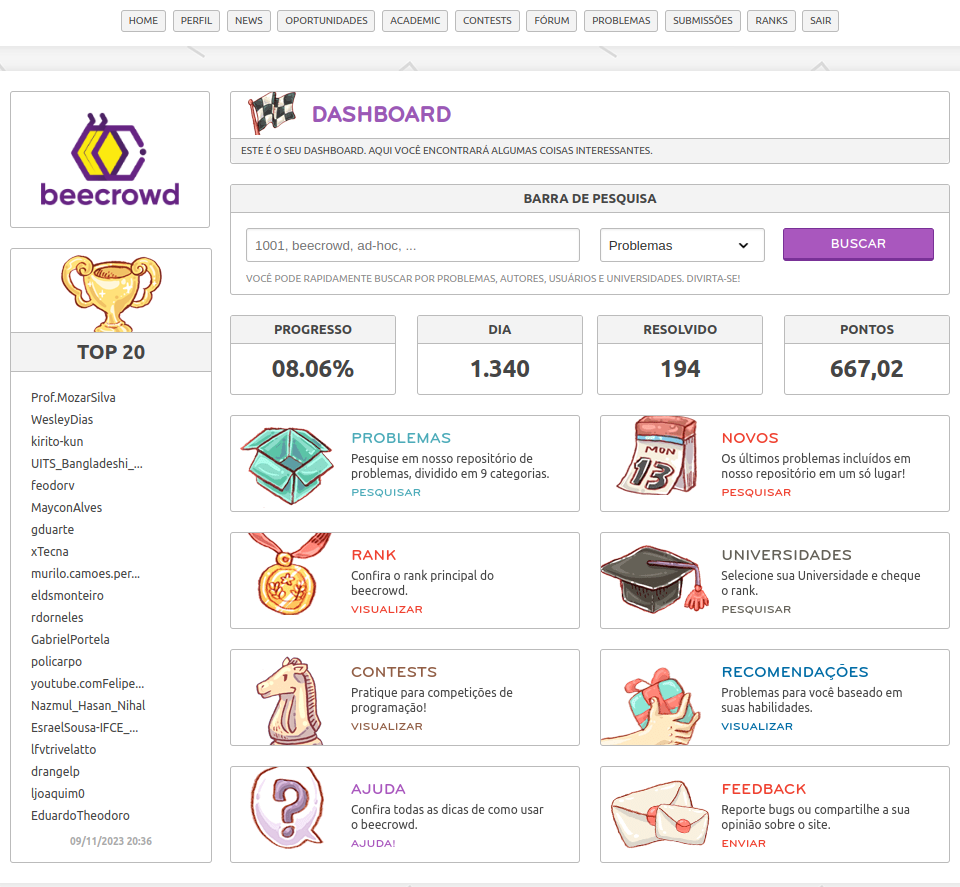
\includegraphics[scale=0.3]{pictures/beecrowd_home.png}
        \fonte{\cite{beecrowd}}
\end{figure}

Além disso, o Beecrowd contém problemas no estilo do ICPC - International Collegiate Programming Contest da ACM, e disponibiliza um juiz online que avalia em tempo real as submissões dos algoritmos dos usuários \cite[p.~350]{berssanettefrancisco}. Os problemas são categorizados por assunto e por nível de dificuldade, e há flexibilidade na escolha da linguagem de programação com a qual se deseja resolver os exercícios \cite[p.~1]{beztonin2012}.

A figura 2 mostra as diferentes categorizações dos exercícios, que são: Iniciante: problemas básicos para quem está iniciando na programação; Ad-Hoc: problemas de simulação, datas e Ad-Hoc no geral; Strings: palíndromos, frequência, ad-hoc, LCS, manipulação de strings; Estruturas e Bibliotecas: filas, pilhas, ordenação, mapas; Matemática: sistemas numéricos, números primos, bigInteger; Paradigmas: programação dinâmica, busca binária, algoritmos gulosos, backtracking; Grafos: flood fill, MST, SSSP, DAG, fluxo máximo, árvores; Geometria Computacional: pontos e linhas, polígonos; e SQL: linguagens de consulta - seleção, inserção, atualização, criação.

\begin{figure}[h!]
	   \centering
            \caption{Portal Beecrowd - Categorias}
            \label{fig:ModeloConceitual}
	   	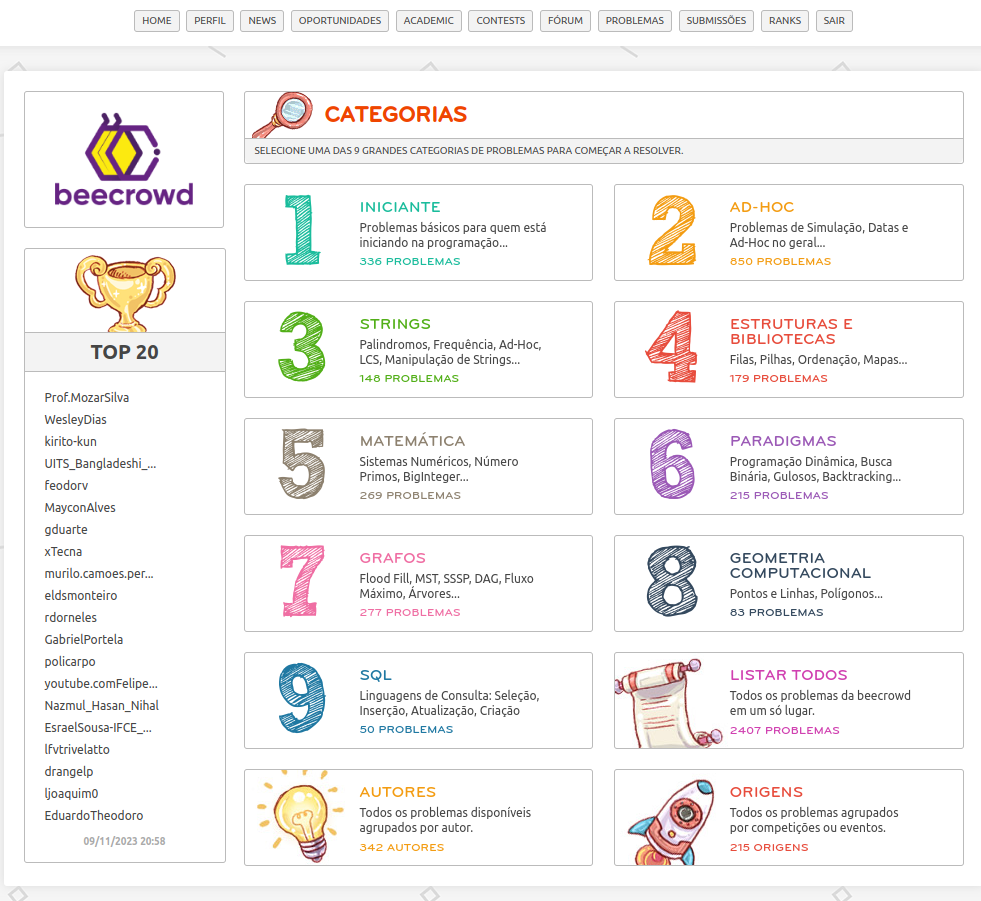
\includegraphics[scale=0.3]{pictures/beecrowd_problemas.png}
        \fonte{\cite{beecrowd}}
\end{figure}

Já na figura 3 estão listados diversos exercícios dentro da categoria Paradigmas, e, para cada problema, há um nível classificado (destacado na imagem com um retângulo azul). O nível representa a dificuldade da questão, e pode variar de 1 até 10, sendo 1 o nível mais fácil, e 10 o nível mais difícil \cite{beecrowd}. Dessa maneira, impede-se que estudantes iniciantes enfrentem frustrações ao tentar resolver problemas que demandam conhecimento mais avançado, prática e técnicas \cite[p.~239]{beztonin2014}.

\begin{figure}[h!]
	   \centering
            \caption{Portal Beecrowd - Exercícios dentro da categoria Paradigmas}
            \label{fig:ModeloConceitual}
	   	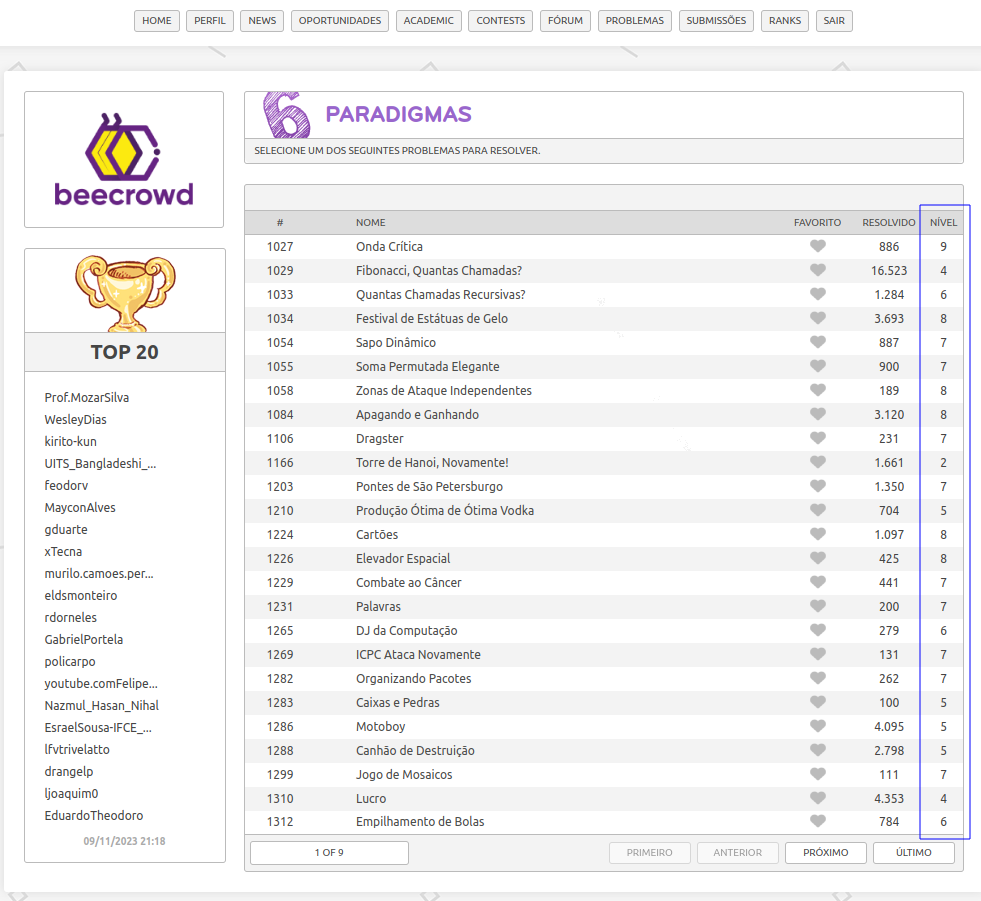
\includegraphics[scale=0.3]{pictures/beecrowd_paradigmas.png}
        \fonte{adaptado de \cite{beecrowd}}
\end{figure}

Ademais, o portal Beecrowd não apenas fornece uma plataforma desafiadora para competições de programação, mas também se destaca como um recurso educacional abrangente. Entre os seus diferenciais, evidenciam-se materiais de estudo, tutoriais sobre algoritmos e programação, e um fórum que facilita a colaboração entre os usuários. Além desses aspectos, o portal foi projetado com características específicas que o tornam uma ferramenta eficaz de apoio às aulas de Algoritmos e Estruturas de Dados. Por meio de problemas que abordam conceitos fundamentais dessas disciplinas, o Beecrowd oferece uma abordagem prática que contribui para uma compreensão mais sólida por parte dos estudantes \cite[p.~2]{beztonin2012}. 

A figura 4 mostra o fórum do exercício 1063 do Beecrowd, que pode ser acessado facilmente em Fórum -> Estruturas e Bibliotecas -> 1063, ou pelo próprio exercício 1063, no seu botão “Fórum”. Nesse fórum, diversas perguntas foram criadas para os alunos conversarem entre si sobre erros e problemas que tiveram.

\begin{figure}[h!]
	   \centering
            \caption{Portal Beecrowd - Fórum do Problema 1063}
            \label{fig:ModeloConceitual}
	   	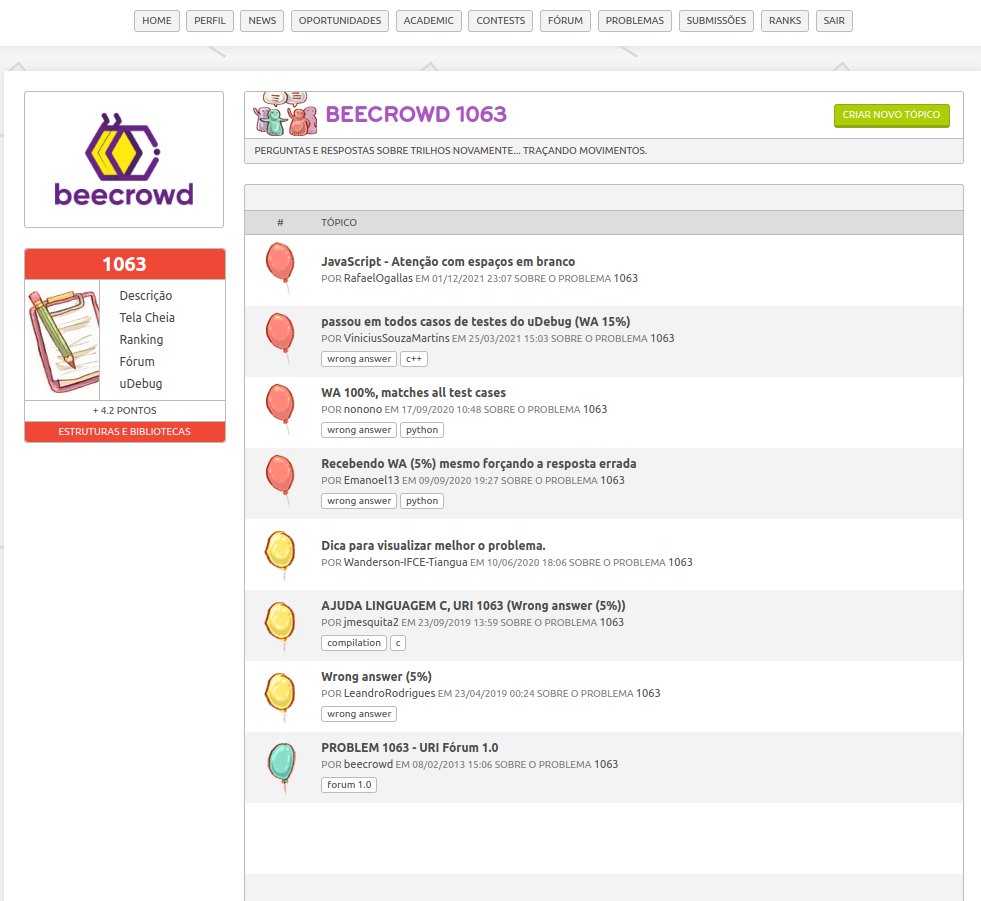
\includegraphics[scale=0.3]{pictures/beecrowd_1063.png}
        \fonte{\cite{beecrowd}}
\end{figure}

Além de ser um recurso fundamental para o aprimoramento das habilidades de programação dos alunos, o Beecrowd disponibiliza recursos diferenciados que se mostram valiosos para professores na área de Tecnologia da Informação. Essas características não apenas enriquecem o ambiente de aprendizado, mas também facilitam o processo de ensino e avaliação em cursos específicos dessa área. Os professores podem, por exemplo, criar disciplinas com alunos e listas de exercícios, separadas por assunto e delimitadas por prazos, caso desejado, e acompanhar a evolução dos alunos \cite[p.~239]{beztonin2014}.

Na figura 5 está a página Academic, do portal Beecrowd, onde alocam-se as disciplinas do usuário. Dentro de cada disciplina se encontram as listas de exercícios disponibilizadas aos alunos pelos professores, bem como algumas orientações aos usuários.

\begin{figure}[h!]
	   \centering
            \caption{Portal Beecrowd - Academic}
            \label{fig:ModeloConceitual}
	   	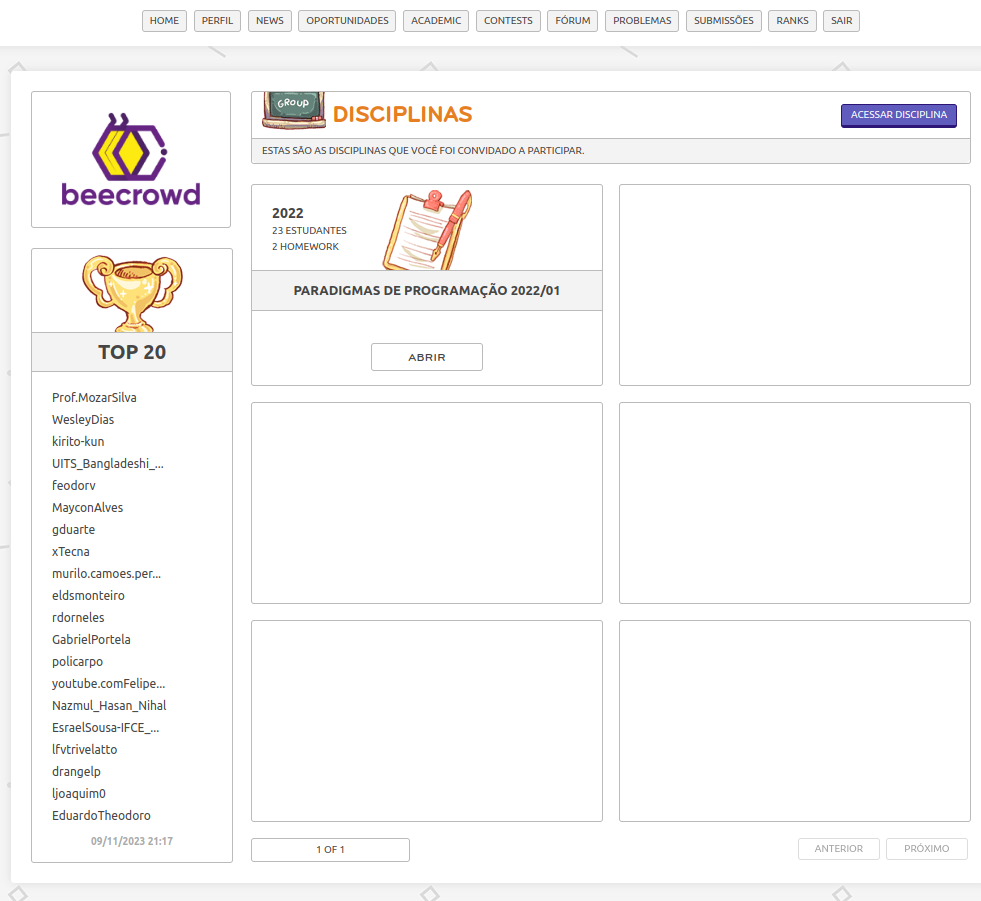
\includegraphics[scale=0.3]{pictures/beecrowd_academic.png}
        \fonte{\cite{beecrowd}}
\end{figure}

Considerando que a construção do Beecrowd foi completamente centrada nas necessidades dos professores e, principalmente, nas necessidades dos alunos \cite[p.~239]{beztonin2014}, ele integra recursos dos melhores portais de programação do mundo e, adicionalmente, oferece funcionalidades exclusivas, como um nível de problemas destinado a iniciantes, um sistema de recompensas por meio de \textit{badges}, e um módulo acadêmico completo para o acompanhamento das listas de exercícios pelos alunos, incluindo o \textit{ranking} dos estudantes por universidade, entre outras inovações \cite[p.~239]{beztonin2014}.

A Figura 5 exemplifica um exercício do Beecrowd, o 1001: Extremamente Básico. Cada exercício é acompanhado por sua descrição, requisitos de entrada para o programa e a saída esperada do algoritmo a ser desenvolvido. Na seção à direita, o usuário pode selecionar a linguagem de programação desejada e utilizar a IDE integrada para desenvolver seu algoritmo. Ao concluir, o usuário deve clicar no botão "Enviar" para que a plataforma avalie sua solução. Após o envio, o aluno é redirecionado para uma tela onde o resultado é exibido na seção "Resposta" (Figura 6).

\begin{figure}[h!]
	   \centering
            \caption{Portal Beecrowd - Exercício 1001}
            \label{fig:ModeloConceitual}
	   	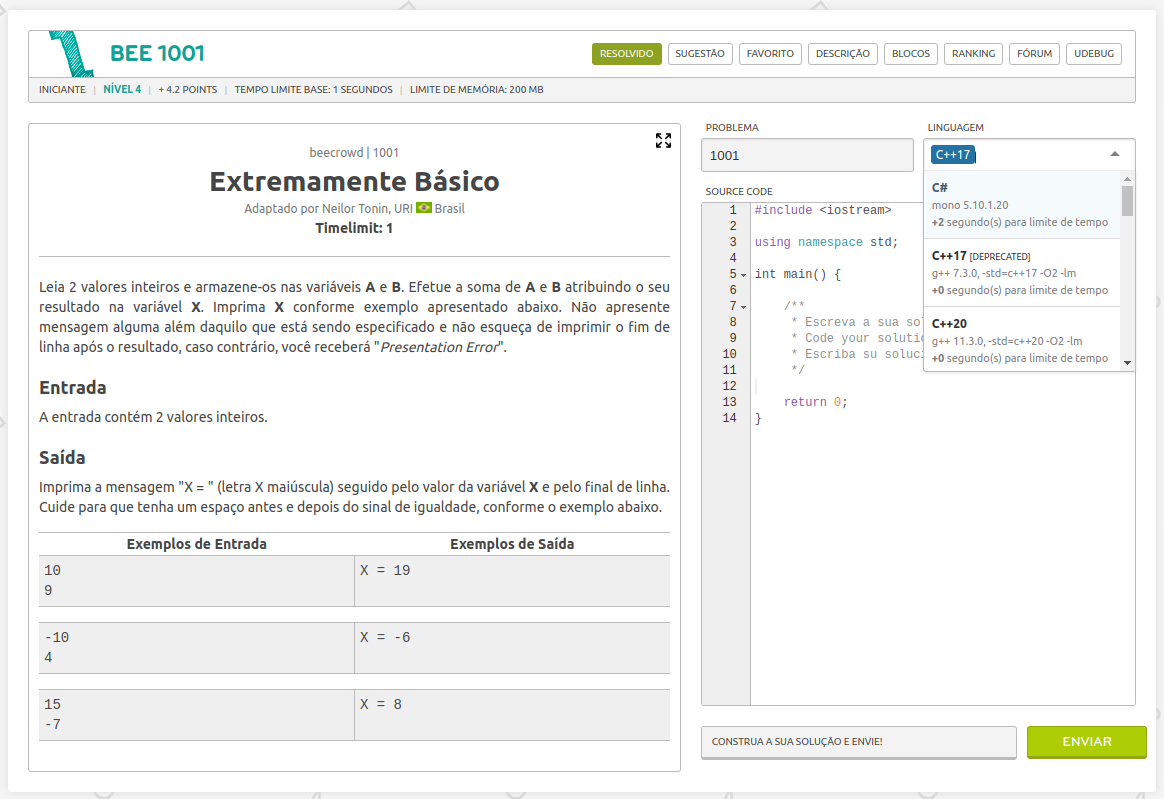
\includegraphics[scale=0.3]{pictures/beecrowd_1001.png}
        \fonte{\cite{beecrowd}}
\end{figure}

\begin{figure}[h!]
	   \centering
            \caption{Portal Beecrowd - Exercício Submetido}
            \label{fig:ModeloConceitual}
	   	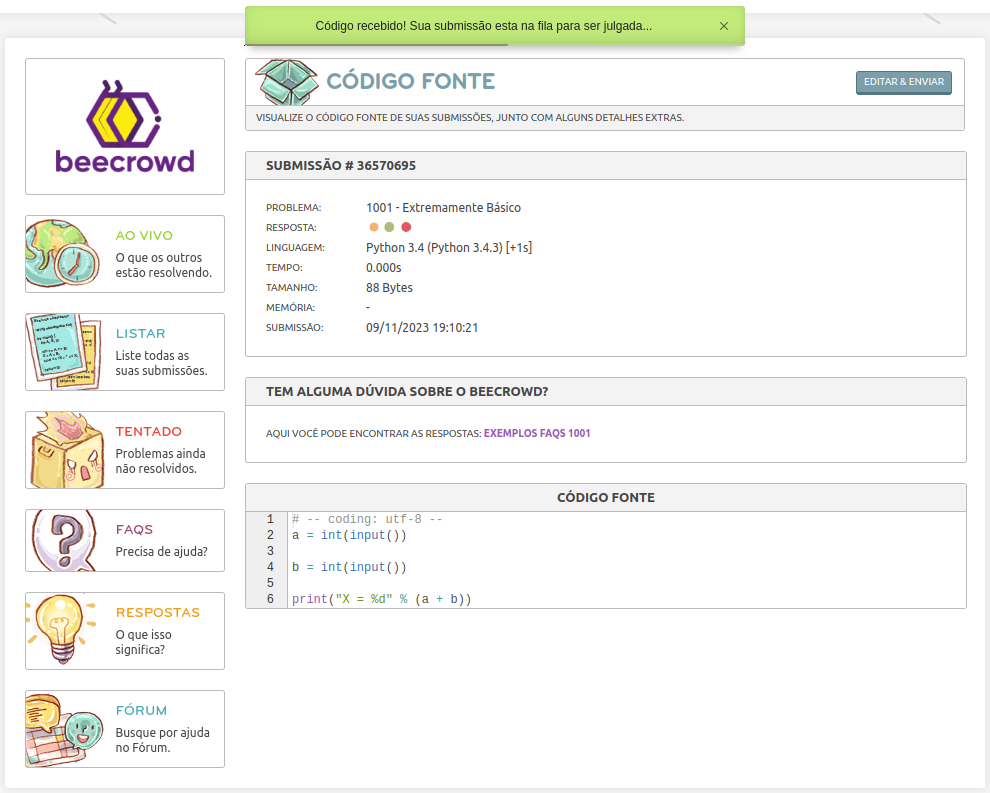
\includegraphics[scale=0.3]{pictures/beecrowd_submetido.png}
        \fonte{\cite{beecrowd}}
\end{figure}

As respostas possíveis do Juíz Online do Beecrowd são: Accepted, Compilation Error, Runtime Error, Time Limited Exceeded, Presentation Error, Wrong Answer, Closed. O significado de cada resposta pode ser encontrado na plataforma, oferecendo ao usuário uma indicação do que pode estar incorreto em seu algoritmo \cite{beecrowd}.

O Beecrowd também possui o ambiente Academic, e é esse ambiente que fornece ao professor diversos recursos \cite{beecrowdacademic}, como:

\begin{itemize}
    \item Criar disciplinas, podendo convidar alunos para participar dela;
    \item Criar listas de exercícios e acompanhar facilmente o progresso de seus estudantes (Veja figura 8), podendo ter uma melhor visão sobre como eles estão aplicando os tópicos apresentados em aula e onde eles estão encontrando dificuldades;
    \item Selecionar exercícios de programação do banco de dados do Beecrowd para essas listas, o qual possui mais de 2.000 problemas distintos;
    \item Visualizar todas soluções enviadas pelos alunos para suas listas de exercícios através de uma organizada linha do tempo;
    \item Definir data de início, prazo e duração das listas, considerando somente as submissões recebidas durante o tempo determinado;
    \item Visualizar \textit{feedback} sobre soluções copiadas entre estudantes e de repositórios online.
\end{itemize}

\begin{figure}[h!]
	   \centering
            \caption{Portal Beecrowd Academic - Progresso dos Alunos}
            \label{fig:ModeloConceitual}
	   	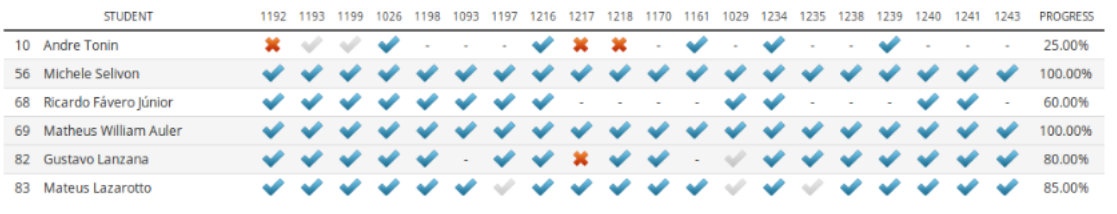
\includegraphics[scale=0.3]{pictures/beecrowd_academic_progresso.png}
        \fonte{\cite[p.~244]{beztonin2012}}
\end{figure}

Por fim, o Beecrowd oferece suporte a várias linguagens de programação e versões, dentre as quais o usuário pode escolher para desenvolver suas soluções. Todas essas linguagens estão listadas abaixo, na figura 9.

\begin{figure}[h!]
	   \centering
            \caption{Portal Beecrowd Academic – Linguagens e Versões}
            \label{fig:ModeloConceitual}
	   	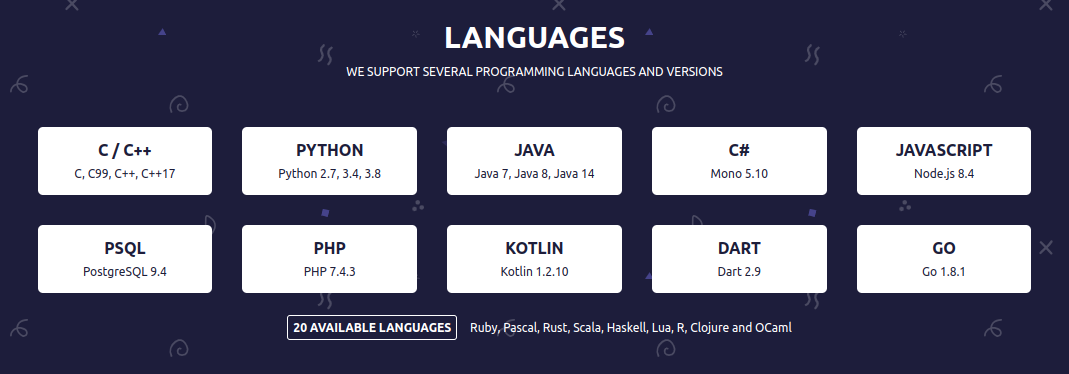
\includegraphics[scale=0.3]{pictures/beecrowd_academic_linguagens.png}
        \fonte{\cite{beecrowd}}
\end{figure}

\section{Boca Online Contest Administrator}

O BOCA Online Contest Administrator é um ambiente utilizado para gerenciar competições que envolvem programação de computadores \cite[p.~22]{galasso}, e foi desenvolvido para ser usado na Maratona de Programação da Sociedade Brasileira de Computação \cite[p.~2]{camposferreira}.

Por ser um juiz online \cite[p.~1]{beztonin2012}, realiza a avaliação automática dos algoritmos submetidos, classificando-os como corretos ou incorretos \cite[p.~22]{galasso}. Ou seja, na competição, a correção dos programas enviados pelos times ocorre de forma online, e o resultado deve ser transmitido ao time o mais rápido possível. Após os competidores concluírem uma questão, enviam-na para o BOCA, que julga a solução fornecida e indica se está correta ou incorreta. Se estiver incorreta, o aluno tem a oportunidade de corrigi-la e submetê-la novamente, ainda durante o tempo da prova, mas sem ter conhecimento específico sobre o erro na questão \cite[p.~4]{camposferreira}. 

A utilização de interfaces web possibilita que o sistema BOCA seja aplicado na organização de competições distribuídas, permitindo que equipes estejam localizadas em qualquer lugar com acesso à internet. Essa abordagem é adequada para simulações e outras modalidades de competições \cite[p.~20]{camposferreira}.
 
Além disso, o BOCA proporciona a flexibilidade de ser utilizado em competições com várias sedes (ou sites), todos operando simultaneamente, com a correção centralizada de submissões e dúvidas. Isso viabiliza competições em larga escala, alcançando regiões distantes de um país, como o Brasil, como evidenciado na Maratona de Programação. A centralização no processamento de submissões e dúvidas é essencial para assegurar igualdade de condições a todos os participantes, independentemente de sua localização, uma vez que tudo é processado pelo mesmo grupo de juízes \cite[p.~10-11]{camposferreira}.

Um benefício adicional do sistema é sua aplicabilidade no contexto de aprendizado, oferecendo suporte a disciplinas que envolvem a submissão e correção de trabalhos de programação \cite[p.~2]{camposferreira}. No entanto, ele foi utilizado por alunos de Ciência da Computação na URI por algum tempo, em sala de aula, para resolver problemas relacionados aos conteúdos abordados. Contudo, a cada semestre, era necessário realizar uma limpeza no site e registrar novos problemas, incluindo todos os seus arquivos de entrada e saída, enunciado, e tempos limites, dependendo da matéria ensinada \cite[p.~1]{beztonin2012}. Os autores \textcite[p.~1]{beztonin2012}. destacaram que lidar com essa quantidade de problemas não é viável, pois o sistema não foi criado para esse propósito. Cada vez que o sistema era limpo, tanto a classificação dos problemas quanto a classificação dos usuários eram perdidas.

Assim, apesar de o BOCA não precisar de cadastro em nenhum portal, e ainda ter acesso a todo código fonte dos exercícios, ele não é a opção ideal para ser o sistema de juiz online utilizado em sala de aula. Ainda assim, o sistema revela-se uma escolha excelente para competições de programação. O crescimento extraordinário dessas competições tem despertado um interesse crescente entre os alunos de cursos de computação no Brasil. Esse interesse é extremamente positivo, pois motiva os alunos a estudarem conceitos fundamentais da computação, tais como estruturas de dados, análise de algoritmos, técnicas e linguagens de programação \cite[p.~11]{camposferreira}.

\section{VPL}

O Virtual Programming Lab (VPL) é um módulo de atividades para o Moodle que gerencia tarefas de programação \cite{vpl}. Suas características distintas incluem a capacidade de editar o código-fonte diretamente no navegador, permitindo aos alunos executar programas de forma interativa sem sair do ambiente Moodle. Tanto alunos quanto professores podem realizar testes para revisar os programas, enquanto a funcionalidade de pesquisa de similaridade entre arquivos auxilia na detecção de plágio. Além disso, o VPL oferece a possibilidade de definir restrições de edição e prevenir a colagem de texto externo, contribuindo para um ambiente acadêmico mais controlado e transparente \cite{vpl}.

Segundo \textcite[p.~1]{rodriguezdelpinoandroyo}, o VPL é um ambiente de desenvolvimento simples para os alunos, oferecendo recursos de avaliação automática. Para os instrutores, funciona como um sistema de gerenciamento do trabalho dos alunos, facilitando a preparação de tarefas, gerenciando envios, verificando plágio e conduzindo avaliações eficientes e flexíveis com base em testes de programas. Além disso, é independente da linguagem de programação utilizada nos exercícios e prioriza questões críticas de segurança.

Para criar uma atividade VPL, é necessário preencher um formulário de configuração básica, seguindo o padrão comum a outros módulos do Moodle. Esse formulário abrange elementos essenciais, como nome da atividade, breve descrição, período de disponibilidade (com datas de início, término e visibilidade), opções de avaliação, agrupamento, entre outros. Adicionalmente, a atividade VPL permite a inclusão de dados específicos, como o número máximo de arquivos a serem enviados, o tamanho máximo desses arquivos, bem como restrições relacionadas à edição, rede, senha, entre outros \cite{vpl}.

Ao concluir o preenchimento do formulário de configuração básica, o criador da tarefa tem a possibilidade de ajustar cinco grupos adicionais de recursos: descrição completa, casos de teste, opções, arquivos solicitados e recursos avançados. Assim, caso o professor queira que os códigos submetidos pelos alunos sejam testados, ele mesmo precisa inserir todos os casos de teste manualmente na tarefa \cite{vpl}.

Assim, sempre que o professor desejar apresentar novas tarefas de programação para suas turmas a cada semestre, será necessário criar uma nova atividade utilizando o VPL, preenchendo integralmente o formulário de configuração básica e incluindo os casos de teste necessários.

\section{CodeRunner}

O CodeRunner é um plugin de código aberto gratuito para o Moodle, projetado para avaliar respostas de programação em várias linguagens. Utilizado principalmente em cursos de programação de computadores, permite que os alunos enviem código em resposta a perguntas específicas e visualizem os resultados dos testes imediatamente. Os professores podem executar programas para avaliar as respostas dos alunos, utilizando uma abordagem adaptativa \cite{coderunner}. Assim, os alunos desenvolvem e testam seu código usando um ambiente de desenvolvimento normal e enviam o código ao CodeRunner por meio de um navegador da Web somente quando acreditam que ele está correto \cite[p.~47]{lobbharlow}.

Funcionando como um tipo de pergunta padrão no Moodle, o CodeRunner foi desenvolvido para integrar-se facilmente com outros tipos de perguntas computadorizadas, como múltipla escolha, numérica, resposta curta, correspondência e até mesmo questões de redação avaliadas por humanos \cite[p.~48]{lobbharlow}. 

Ao contrário do VPL, o CodeRunner opera no modo de teste adaptativo, onde os alunos podem verificar imediatamente se o código passa nos testes definidos na pergunta. Eles podem corrigir e reenviar o código, geralmente com uma pequena penalidade. A avaliação é baseada nos casos de teste aprovados pelo aluno \cite{moodle}.

 Adicionalmente, o CodeRunner proporciona um sistema flexível de penalidades, permitindo que os criadores ajustem a avaliação conforme o contexto. Por exemplo, é possível configurar algumas perguntas sem penalidades para reenvios, outras que concedem um ou dois envios gratuitos antes de aplicar uma penalidade incremental de 10\% para cada tentativa subsequente errada, e ainda outras que impõem uma penalidade de 100\% mesmo para um único reenvio equivocado. Vale ressaltar a alta escalabilidade do CodeRunner: ele acomoda desde questões simples de codificação até tarefas significativamente complexas \cite[p.~48]{lobbharlow}.
 
Atualmente, o CodeRunner é compatível com Python2 (considerado obsoleto), Python3, C, C++, Java, PHP, JavaScript (NodeJS), Octave e Matlab. A arquitetura permite a fácil expansão para outras linguagens \cite{moodle}.

Para garantir a segurança, o CodeRunner necessita do software sandbox ("Jobe") instalado em uma máquina separada com medidas adequadas de segurança. Recomenda-se o uso de um servidor Moodle separado para questionários baseados no CodeRunner, especialmente em testes e exames finais, tanto por motivos de carga quanto para que vários recursos de comunicação do Moodle, como bate-papo e mensagens, possam ser desativados sem afetar outras turmas \cite{coderunner}.

Assim como no VPL, é necessário que o criador da pergunta configure seus detalhes e seus casos de teste \cite{coderunner}.

A Universidade de Canterbury utiliza o CodeRunner para ministrar cursos de programação em Python, C, Octave e Matlab. Esse plugin é especialmente eficaz em cursos introdutórios de programação, proporcionando prática intensiva com pequenos problemas de programação que ensinam diversas construções e técnicas de linguagem. No entanto, o CodeRunner também é aplicável em níveis mais avançados, sendo utilizado em cursos teóricos de ciência da computação, inteligência artificial (com programação em Clojure) e programação na web para avaliação de sites desenvolvidos pelos alunos \cite[p.~48]{lobbharlow}.

\section{Moodle}

“Moodle é uma plataforma de aprendizagem projetada para fornecer a educadores, administradores e alunos um único sistema robusto, seguro e integrado para criar ambientes de aprendizagem personalizados” \cite{moodle}. Ou seja, o Moodle é um Sistema de Gerenciamento de Aprendizagem (LMS) poderoso e altamente extensível \cite{moodle}. 

Desenvolvido pelo projeto Moodle, a plataforma possui uma interface web amplamente acessível, permitindo que estudantes, tutores e administradores realizem tarefas diárias de qualquer lugar do mundo. Com suporte para várias opções técnicas, garante bom desempenho, sendo utilizado por instituições de destaque, como o Open Polytechnic da Nova Zelândia, que atende mais de 45.000 estudantes e oferece 6.500 cursos registrados \cite{moodle}. 

Projetado e auditado para segurança, o Moodle conta com funções específicas para administradores, professores, alunos e visitantes, com um conjunto claro de privilégios. Comprometido com a segurança e privacidade, mantém controles atualizados contra acesso não autorizado, perda de dados e uso indevido. Pode ser implantado em nuvem privada segura ou servidor para controle total \cite{moodle}. 

Reconhecido globalmente em ambientes de aprendizagem, está disponível em mais de 60 idiomas e é utilizado por instituições renomadas, incluindo London School of Economics, Shell e Microsoft, contando com mais de 213 milhões de usuários em nível acadêmico e empresarial \cite{moodle}. 

O Moodle oferece um conjunto robusto de ferramentas centradas no aluno e ambientes colaborativos para facilitar o ensino e aprendizagem. Com uma interface simples, é fornecido gratuitamente como software de código aberto sob a GNU General Public License, permitindo adaptação para projetos comerciais e não comerciais sem custos de licenciamento. Sua constante revisão atende às necessidades em evolução dos usuários e permite escalabilidade para turmas pequenas e grandes organizações \cite{moodle}. 

Como software de código aberto, possibilita personalização e adaptação, com estrutura modular e design interoperável para o desenvolvimento de plugins e integração de aplicativos externos. Proporciona flexibilidade excepcional para apoiar a aprendizagem combinada e cursos totalmente online, configurável conforme necessário e integrando facilmente diversas ferramentas colaborativas \cite{moodle}. 

Contando com forte apoio de uma comunidade global ativa, equipe de desenvolvedores dedicados e parceiros certificados, o Moodle recebe atualizações rápidas, correções de bugs e melhorias em lançamentos significativos a cada seis meses \cite{moodle}.

Atualmente, diversas instituições educacionais buscam modernizar seus sistemas de aprendizagem para facilitar o acesso ao conhecimento. Nesse contexto, o ambiente Moodle tem se destacado como uma escolha frequente. O Moodle adota o conceito construcionista social de educação, conforme destacado por \cite[p.~22]{galasso}. Esse enfoque pedagógico enfatiza as demandas contemporâneas por métodos de ensino mais dinâmicos e participativos.

\subsection{Características Gerais do Moodle}

O Moodle, flexível e de fácil instalação em plataformas que suportam PHP, exige apenas uma base de dados, de qualquer marca. Destaca-se por sua ênfase na segurança, implementando verificações rigorosas em formulários, validação de dados, e codificação de cookies. Também permite que um site Moodle suporte milhares de cursos, estes podendo ser categorizados e pesquisados.

\subsubsection{Administração do site}

\begin{itemize}
    \item O site é administrado por um usuário administrador, permitindo ajustes de aparência por meio de extensões (plug-ins) de temas;
    \item Oferece suporte a extensões de módulos de atividade e pacotes de idiomas, possibilitando compatibilidade com mais de 60 idiomas; 
    \item O código PHP, licenciado sob GPL, é claro e facilmente modificado para atender às necessidades individuais.
\end{itemize}

\subsubsection{Administração dos usuários}

\begin{itemize}
    \item Objetiva reduzir a intervenção do administrador, suportando diversos mecanismos de autenticação, como email, LDAP, IMAP, POP3, NNTP, e base de dados externa;
    \item Permite que cada pessoa possua uma única conta para todo o servidor, com diferentes acessos configuráveis; 
    \item Uma conta de administrador controla a criação de cursos e cria professores através da inscrição de usuários aos cursos;
    \item Somente é permitida a uma conta de criador de cursos criar e dar aula nos cursos;
    \item Os professores podem acrescentar uma “chave de inscrição” a seus cursos para manter fora os não inscritos. Eles podem fornecer essa chave diretamente ou através do email particular de cada um;
    \item Os professores podem incluir e excluir alunos manualmente;
    \item Cada usuário pode especificar faixas de horário para que cada compromisso seja ajustado a esses horários, e escolher o idioma de interface.
\end{itemize}

\subsubsection{Administração do Curso}

\begin{itemize}
    \item Professores têm controle total sobre os parâmetros do curso, podendo restringir outros professores;
    \item Oferece flexibilidade na composição de atividades, como fóruns, jornais, questionários, recursos, pesquisas de opinião, tarefas e chats. 
    \item Todas as notas para os fóruns, jornais, questionários e tarefas podem ser vistas em uma página;
    \item Rastreamento detalhado dos usuários, relatórios de atividade com gráficos, e história detalhada do envolvimento de cada aluno, como postagens.
\end{itemize}

\subsection{LTI External tools}

Ferramentas Externas LTI do Moodle são aplicativos adicionais que você pode integrar curso, como conteúdo interativo, atividades ou avaliações. Os professores podem vincular essas atividades diretamente na página do curso no Moodle, e os alunos podem acessá-las sem sair do curso no Moodle ou precisar fazer login em um sistema diferente. Onde disponível, e dependendo de cada ferramenta, os professores também podem fazer com que as notas sejam enviadas de volta ao Moodle \cite{moodle}.

A conexão entre o Moodle e essas ferramentas é feita através do padrão Learning Tools Interoperability (LTI), que integra plataformas de aprendizado com ferramentas de aprendizado para criar uma experiência de aprendizado mais rica e contínua. Essencialmente, o padrão LTI permite uma troca segura e bidirecional de informações entre o Moodle e ferramentas de aprendizado externas \cite{moodle}. 

O administrador tem permissão para gerenciar Ferramentas Externas LTI, podendo adicionar novas ferramentas aos seus cursos usando o botão ‘Adicionar ferramenta’ na página de Ferramentas Externas LTI \cite{moodle}.

As ferramentas adicionadas no nível do curso aparecerão na sua lista de atividades por padrão, sendo possível removê-las da lista de atividades acessando a página do curso > Mais > Ferramentas Externas LTI e desmarcando-as na coluna ‘Mostrar na lista de atividades’ \cite{moodle}.

Para configurar uma ferramenta externa LTI, é necessário ir até "Configurações da ferramenta", fornecer um nome para a ferramenta (e, opcionalmente, uma descrição). Para preencher os outros campos nesta seção, incluindo a versão LTI, deve-se seguir as instruções do fornecedor da sua ferramenta. Se a ferramenta não fornecer informações sobre algumas dessas configurações, você pode deixá-las em branco \cite{moodle}.

De acordo com \textcite{moodle}, os campos a serem preenchidos para configuração de uma ferramenta externa LTI são:

\begin{itemize}
    \item URL da ferramenta – Esta é a URL para conectar ao site. Se o site Moodle usar SSL (estiver em HTTPS), só é possível usar uma ferramenta que também use SSL. É necessário certificar-se de que a URL da ferramenta tenha HTTPS antes de tentar usá-la;
    \item Versão LTI – A versão LTI da ferramenta que está sendo adicionada; 
    \item Chave do consumidor – Isso informa ao site LTI compatível conectado que o Moodle está autorizado a se conectar. O "fornecedor da ferramenta", ou seja, o gerente do site LTI compatível conectado, fornecerá essa chave. Se o administrador estiver apenas vinculando a uma ferramenta sem acesso seguro ou compartilhamento de notas, não será necessário uma chave do consumidor. Se estiver vinculando a um curso ou atividade de outro site Moodle, o administrador pode adicionar qualquer chave do consumidor;
    \item Segredo compartilhado – Este é o "senha" para conectar à ferramenta – o site LTI compatível;
    \item Parâmetros personalizados – Na maioria das vezes, esse campo pode ficar em branco. O fornecedor da ferramenta pode usar isso para permitir que o administrador exiba um recurso específico;
    \item Contêiner de lançamento padrão – Esta é a forma como a ferramenta externa será exibida;
    \item Incorporar – O conteúdo aparecerá dentro da página de atividade onde a ferramenta é usada, sem afastar os usuários da página, mas ocultando quaisquer blocos que o curso possa ter;
    \item Incorporar sem blocos – O conteúdo será exibido na guia ou janela existente. Os usuários terão que navegar de volta para o curso usando o botão ‘Voltar’ assim que terminarem;
    \item Janela existente – O conteúdo será exibido na guia ou janela existente. Os usuários terão que navegar de volta para o curso usando o botão ‘Voltar’ assim que terminarem;
    \item Nova janela – A ferramenta externa será aberta em uma nova janela. (Uma nova janela ou guia será aberta com a ferramenta externa e a janela do navegador antiga contendo a página do curso não será alterada);
    \item URL de seleção de conteúdo – A URL de Seleção de Conteúdo será usada para abrir a página de seleção de conteúdo do fornecedor da ferramenta. Se estiver vazia, a URL da ferramenta será usada;
    \item URL do ícone – É possível exibir um ícone diferente do ícone padrão da Ferramenta Externa inserindo sua URL nesse campo;
    \item URL do ícone seguro – É possível inserir URL de um ícone diferente aqui se os alunos estiverem acessando o Moodle com segurança via SSL
\end{itemize}

\section{LTI}

A especificação Learning Tools Interoperability (LTI) foi inicialmente introduzida como Basic LTI em maio de 2010 pelo IMS Global Learning Consortium (agora conhecida como LTI 1.0). Desde então, essa especificação ganhou ampla aceitação como um método simples, mas eficaz, para integrar conteúdos e produtos de terceiros aos Ambientes Virtuais de Aprendizagem (VLEs). Hoje em dia, ela faz parte integral dos principais VLEs, como o Moodle, Blackboard Learn 9, Desire2Learn e o Canvas da Instructure \cite[p.4]{vickers}.

Assim, o padrão LTI permite uma troca segura de dados entre o LMS e ferramentas de aprendizagem externas, centralizando o acesso a conteúdo interno e externo, oferecendo uma experiência de aprendizado consistente, eliminando a necessidade de múltiplos logins para diferentes plataformas \cite{verdaguer}.

\section{Sistema Especialista}

De acordo com \textcite{jimmysingla}, um sistema especialista é um conjunto de programas que manipula conhecimento para resolver problemas em um domínio especializado que exige a expertise humana. Já \textcite{markobohanec} definem sistemas especialistas como sistemas inteligentes de informação que imitam, em certo grau, o comportamento de um especialista humano no domínio em questão.

Também chamados de sistemas baseados em conhecimento, esses programas de computador armazenam o conhecimento específico de um ou mais especialistas humanos \cite{jimmysingla}. Os principais componentes de um sistema especialista são a base de conhecimento e a máquina de inferência. A base de conhecimento armazena informações sobre um domínio específico de problemas, enquanto a máquina de inferência utiliza esse conhecimento para resolver problemas indicados pelo usuário, gerando explicações orientadas a ele sobre as soluções propostas \cite{markobohanec}. 

Assim, a base de conhecimento contém o conhecimento do domínio necessário para resolver problemas, geralmente na forma de regras, um dos paradigmas mais populares para a representação de conhecimento; e o motor de inferência é o núcleo do sistema, responsável por gerar conclusões a partir da base de conhecimento através de inferência ou raciocínio \cite{jimmysingla}. Portanto, um sistema especialista para tomada de decisão precisa estabelecer uma base de conhecimento apropriada e usá-la para o cálculo de utilidade \cite{markobohanec}.

O autor \textcite{jimmysingla} ressaltou que as principais características de um sistema especialista incluem interface com o usuário, representação de dados, inferência, capacidade de explicação e habilidade de lidar com incertezas. Entre as vantagens, esse tipo de sistema oferece resposta rápida, maior confiabilidade, redução de custos e de erros, uso de múltiplas expertises, banco de dados inteligente e mitigação de riscos. Contudo, o sistema apresenta algumas limitações, como a ausência de senso comum, a incapacidade de responder a casos excepcionais e a dificuldade de adaptação a ambientes em constante mudança \cite{jimmysingla}. 

\subsubsection{Prolog}

De acordo com \textcite{keithclark}, o Prolog, uma linguagem de programação baseada na lógica de predicados proposta por Kowalski, foi desenvolvida pelo grupo de Alain Colmerauer em Marselha. Sua implementação mais conhecida é o compilador DEC-10 de Edimburgo, que apresenta eficiência comparável à de LISP, mas com maior suporte a inferências, essencial em sistemas especialistas. Em Marselha, é aplicada no processamento de linguagem natural, enquanto em Edimburgo é usada para planejamento, resolução de problemas e desenvolvimento de compiladores \cite{keithclark}.

\textcite{keithclark} também explicam que, na Hungria, a linguagem de programação Prolog é amplamente utilizada em sistemas especialistas, especialmente na farmacologia, incluindo previsão de atividades biológicas e interações medicamentosas. Experiências como um sistema de diagnóstico de falhas no Imperial College demonstram o potencial de Prolog para sistemas especialistas, incentivando novas aplicações \cite{keithclark} .

Já \textcite{stuartrussel} mostram que o Prolog é, de longe, a linguagem de programação lógica mais amplamente utilizada, sendo popular para prototipação rápida e manipulação simbólica, como no desenvolvimento de compiladores e análise de linguagem natural. Além disso, diversos sistemas especialistas foram implementados em Prolog para áreas como direito, medicina \cite{jimmysingla}, finanças e outros domínios especializados \cite{stuartrussel}.

Além disso, o Prolog é ideal para desenvolver serviços Web robustos devido à sua semântica segura e gerenciamento automático de memória \cite{wielemaker}.

Programas em Prolog consistem em conjuntos de cláusulas escritas com a seguinte notação:  as variáveis são indicadas por letras maiúsculas, enquanto as constantes são escritas em letras minúsculas; e  a estrutura das cláusulas, ao invés de A ∧ B ⇒ C, utiliza-se C :- A, B, com vírgulas separando os elementos da conjunção \cite{stuartrussel}.

\subsubsection{SWI-Prolog}

O SWI-Prolog é uma implementação de Prolog baseada em um subconjunto da WAM (Warren Abstract Machine), que possui um ambiente robusto de desenvolvimento, priorizando compatibilidade, portabilidade, escalabilidade e estabilidade \cite{wielemakerswiprolog}. 

O SWI-Prolog, projeto de código aberto, foi moldado para desenvolver protótipos de pesquisa, especialmente em sistemas interativos e que exigem intensivo uso de conhecimento \cite{wielemakerswiprolog2}. Além do sistema básico, foram integrados ao SWI-Prolog várias interfaces e bibliotecas de restrições. Assim, o SWI-Prolog atua como uma ferramenta integradora e versátil, permitindo a interação com diversos recursos externos e apoiando inovações da comunidade Prolog \cite{wielemakerswiprolog2}.

Como o SWI-Prolog inclui uma extensa gama de biblioteca, que permite integração com gráficos (XPCE), bancos de dados, redes, outras linguagens de programação e diferentes formatos de documentos, ele é uma escolha poderosa para o desenvolvimento de aplicações que requerem integração e lógica sofisticada, mantendo uma estrutura de código organizada e eficiente \cite[p.~1]{wielemakerswiprologversion7}.

Outra vantagem do SWI-Prolog é a disponibilidade de bibliotecas para servidor HTTP, o que facilita o desenvolvimento de controles de servidor \cite{wielemakerswish}. Essas bibliotecas foram projetadas para que o Prolog se comunique com outros componentes de aplicações Web por meio do protocolo HTTP padrão. Com isso, a arquitetura é capaz de gerenciar protocolos de transferência e realizar parsing, representação e geração dos principais formatos de documentos Web, como HTML, XML e RDF, de forma integrada e padronizada \cite{wielemaker}.

\section{WEB API}

Os Web Services (Serviços da Web) são servidores da Web dedicados a propósitos específicos, atendendo às demandas de um site ou de outros aplicativos. Para interagir com esses serviços, os programas clientes utilizam Interfaces de Programação de Aplicações (APIs). Em essência, uma API expõe conjuntos de dados e funções, facilitando a comunicação entre programas de computador e viabilizando a troca de informações. Uma API da Web representa a interface de um serviço da Web, sendo responsável por receber e responder diretamente às solicitações dos clientes \cite[p.~5]{masse}.

A interação com uma Web API envolve a realização de solicitações (requests) por meio dos protocolos de comunicação HTTP ou HTTPS. Essas solicitações são essenciais para a comunicação entre programas clientes e serviços da Web, permitindo a troca de informações de maneira estruturada \cite[p.~18-20]{richardson}. 

Quando um programa cliente envia uma solicitação para uma Web API, ele está requisitando a execução de uma operação específica ou a obtenção de dados do serviço da Web. Essa solicitação é processada pelo serviço da Web, que fornece uma resposta (response) ao cliente. O formato comum para a estruturação dessas respostas é o JSON (JavaScript Object Notation), um padrão amplamente adotado para representar estruturas de dados \cite[p.~19-21]{richardson}. 

Essa dinâmica de solicitação e resposta é a base do funcionamento de uma Web API. As solicitações podem conter parâmetros que informam ao serviço da Web sobre a operação desejada, e a resposta contém os dados solicitados ou uma confirmação da operação realizada. Esse modelo facilita a integração de sistemas e a comunicação entre diferentes componentes de software, sendo fundamental em ambientes de desenvolvimento web e integração de aplicativos \cite[p.~20-23]{richardson}.
